\section{Linguistic Analysis}

Sawicki et al. 2023's survey \cite{sawicki_state_2023} tells us that English is by far the most represented language in the field of natural language processing. Fortunately, French and Italian are still in the top eight (figure \ref{fig:lanpop}), so finding libraries already capable of handling them should be easy enough. It is worth noting that results could be biased since the authors looked for papers written in English.

\begin{figure}[h]
  \centering
  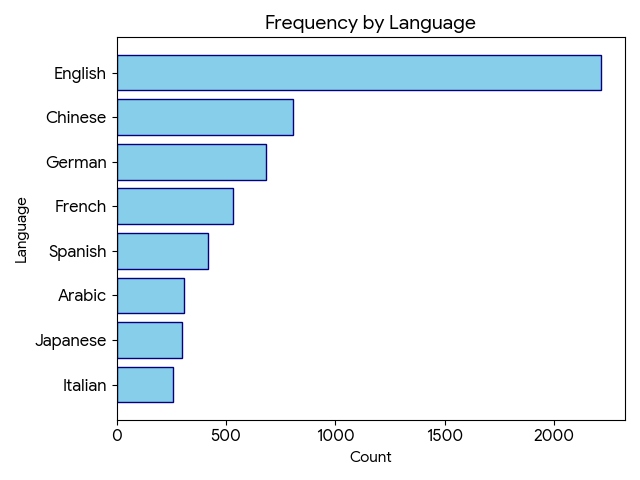
\includegraphics[width=.7\linewidth]{images/sawicki_languagesPopularity.png}
  \caption{Most popular languages in the field of Natural Language Processing \cite{sawicki_state_2023}}
  \Description{English is at 2000 count popularity, Chinese second most popular at 700. Italian least popular at 300.}
  \label{fig:lanpop}
\end{figure}

The pipeline for pre-processing is quite standard and involves, among other steps, removing stop words, part-of-speech tagging, tokenization and lemmatization, as well as building text embeddings. 

\textbf{FastText}\footnote{FastText is a lightweight library for efficient text classification and representation learning: \url{https://fasttext.cc/}.} is an open-source, free, lightweight library that allows users to learn text representations and text classifiers; it gained significant popularity due to its performance in computing text embeddings. 

\textbf{LLM2Vec} \cite{behnamghader_llm2vec_2024} is a recipe to convert decoder-only LLMs into text encoders so that they can be used to generate state-of-the-art text embeddings.

\textbf{Stanza}\footnote{Stanza – A Python NLP Package for Many Human Languages: \url{https://stanfordnlp.github.io/stanza/index.html}.} is a collection of accurate and efficient tools for the linguistic analysis of many human languages. Starting from raw text, Stanza divides it into sentences and words, and can then recognize parts of speech and entities, perform syntactic analysis, and more. Stanza brings state-of-the-art NLP models to the languages of your choosing.

\textbf{spaCy}\footnote{spaCy, Industrial-Strength Natural Language Processing: \url{https://spacy.io/}.} is another well-known and powerful NLP library for Python that supports multiple languages. It also supports tokenization, part-of-speech tagging, dependency parsing, sentence segmentation, text classification, and lemmatization. It supports multi-task learning with pretrained transformers, includes pretrained word vectors, supports custom models in PyTorch and TensorFlow, and has built-in syntax visualizers.

\textbf{simplemma}\footnote{simplemma is a lightweight toolkit for multilingual lemmatization and language detection: \url{https://pypi.org/project/simplemma/}.} is also worth mentioning as a lightweight Python lemmatizer.

\textbf{textacy}\footnote{textacy: NLP, before and after spaCy. \url{https://pypi.org/project/textacy/}.} is a Python library for performing a variety of natural language processing (NLP) tasks. It is built on spaCy and intended to be used both before (pre-processing step) and after (NLP step) it. It assesses text complexity with the Flesch-Kincaid readability test and text diversity with the Type-Token Ratio. 

Text complexity can also be measured with \textbf{TRUNAJOD}\footnote{TRUNAJOD: A text complexity library for text analysis built on spaCy. \url{https://trunajod20.readthedocs.io/en/latest/}.}, another spaCy-based Python library that implements synonym overlap, coherence between sentences, and other metrics. 

Regarding populism and hate speech classification, there are many transformer-based models available from \textbf{Hugging Face}\footnote{Hugging Face, Inc., is an American company based in New York City that develops computational tools for building applications using machine learning. Its transformers library, built for natural language processing applications, and its platform allow users to share machine learning models and datasets and showcase their work. \url{https://huggingface.co/}}. Some examples follow:

\begin{itemize}
    \item English: \url{https://huggingface.co/Hate-speech-CNERG/dehatebert-mono-english};
    \item French: \url{https://huggingface.co/Hate-speech-CNERG/dehatebert-mono-french};
    \item Italian: \url{https://huggingface.co/Hate-speech-CNERG/dehatebert-mono-italian}.
\end{itemize}

There are transformer models based on RoBERTa for both hate speech and populism classification. For example, the following is a 0.4 billion parameter model based on Trump speeches: \url{https://huggingface.co/coastalcph/roberta-large-ft-trump-populism}.

Hate speech can also be detected with the Python library \textbf{HateSonar}\footnote{HateSonar: Hate Speech Detection. \url{https://pypi.org/project/hatesonar/}.}, which uses a BERT-based model.

\subsection{Speech To Text}

Since there are plenty of video and audio speeches publicly available, they could be integrated into the corpus after transcribing them into text. This can be achieved with libraries such as \textbf{SpeechRecognition}\footnote{SpeechRecognition, a Python library for performing speech recognition with support for several engines and APIs, online and offline. \url{https://pypi.org/project/SpeechRecognition/}.}, which supports several different engines and APIs both online and offline, or OpenAI's \textbf{Whisper}\footnote{Whisper is a general-purpose speech recognition model. \url{https://github.com/openai/whisper}.} library. Whisper is a Transformer sequence-to-sequence model trained on various speech processing tasks, including multilingual speech recognition, speech translation, spoken language identification, and voice activity detection. It comes in six different model sizes; the "small" model requires approximately 2GB of VRAM, making it easy to run locally.

Whisper's performance varies depending on the language. Italian is the fourth best-performing language with a WER\footnote{Word Error Rate (WER) is a common metric for the performance of speech recognition or machine translation systems. It is measured as an error rate percentage for compared sentences.} of 5.5\%. English follows at 9.3\% and French at 10.8\% \cite{radford_robust_2022}. The worst-performing language is Albanian with a WER of 55.7\%.

Whisper can be used both in Python scripts and via a command-line interface.